\documentclass{article}
\usepackage[utf8]{inputenc}
\usepackage[T2A]{fontenc}
\usepackage[russian]{babel}
\usepackage{graphicx}
\usepackage{amsmath}
\usepackage{amssymb}
\usepackage{bm}
\usepackage[thinc]{esdiff}
\usepackage{mathtools}
\usepackage{breqn}
\usepackage{amsthm}
\usepackage{amsfonts}
\usepackage{bbm}

%Русская традиция
\renewcommand{\leq}{\leqslant}
\renewcommand{\geq}{\geqslant}
\renewcommand{\phi}{\varphi}
\DeclareMathOperator*{\argmax}{argmax}

\theoremstyle{definition}
\newtheorem{definition}{Определение}
\newtheorem*{definition*}{Определение}
\theoremstyle{theorem}
\newtheorem{theorem}{Теорема}
\theoremstyle{remark}
\newtheorem{remark}{Замечание}
\theoremstyle{theorem}
\newtheorem{corollary}{Следствие}
\theoremstyle{example}
\newtheorem{example}{Пример}
\theoremstyle{theorem}
\newtheorem{statement}{Утверждение}
\theoremstyle{theorem}
\newtheorem{alg}{Алгоритм}
\theoremstyle{theorem}
\newtheorem{sug}{Предположение}
\theoremstyle{theorem}
\newtheorem{lemma}{Лемма}

\begin{document}

\tableofcontents

\newpage

\section{Решающие деревья}
	Пусть $\mathbf X\in\mathbb R^{n\times k}$~--- матрица данных, $n$~--- число индивидов, $k$~--- число признаков, $Y\in\mathbb R^n$~--- вектор отклика, $X_i$~--- вектор признака, $i\in1:k$.
	\begin{definition}
		Дерево решений~--- бинарное дерево $(V,E)$, в котором каждой $v\in V$, не являющейся листом соответствует функция, являющаяся предикатом $\beta_v:X\to\{0,1\}$, а каждому листу $l\in V$ соответствует прогноз $f_l:X\to Y$.
	\end{definition}
	\begin{figure}[h!]
			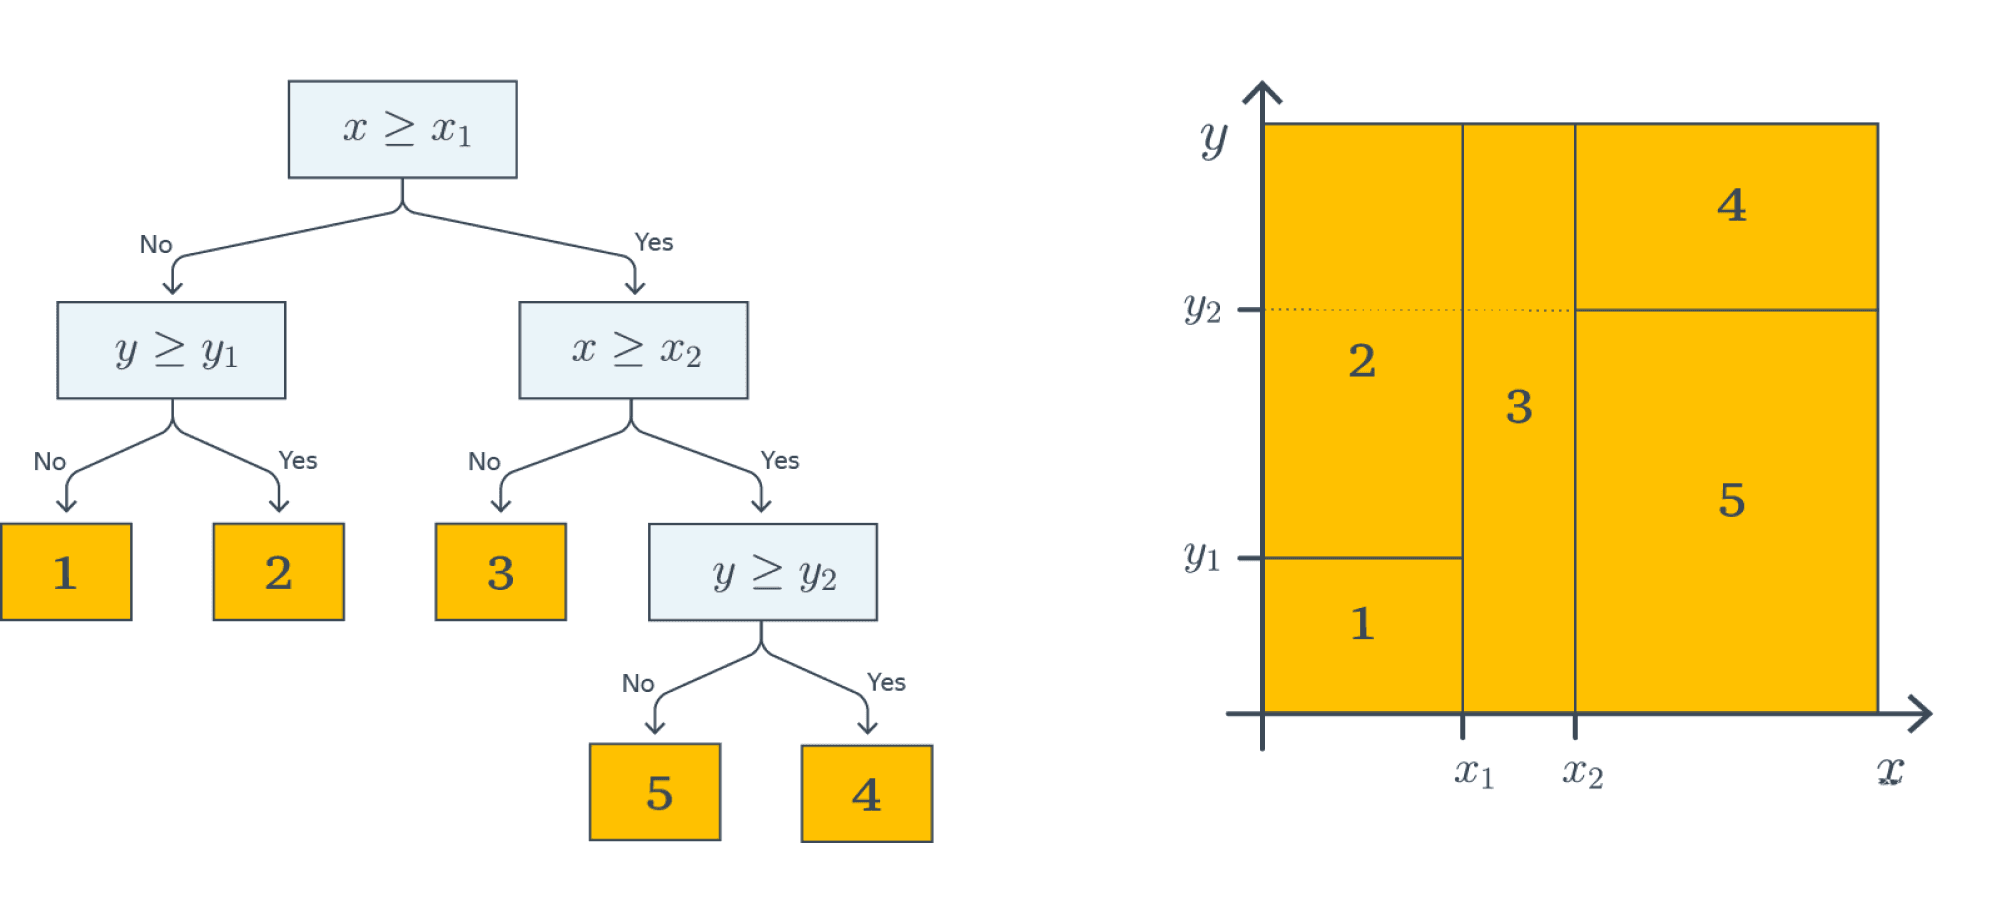
\includegraphics[width=\textwidth]{bintree_class.png}	\caption{Пример дерева решений}
	\end{figure}
	
	Деревья решений можно применять для классификации и регрессии.
	\subsection{Задача регрессии}
		Разобьём всевозможные значение $X_i$, $i\in1:k$ на $J$ непересекающихся множеств $\{R_j\}_{j=1}^J$, $R_j\in\mathbb R^k$. Предсказание для $x\in X$ равно $$f(x)=\sum\limits_{j=1}^Jc_j\mathbbm{1}(x\in R_j).$$
		
		Выбирать набор $R_j$ будем решая оптимизационную задачу минимизации суммы квадратов остатков $$\mathrm{RSS}=\sum\limits_{j=1}^J\sum\limits_{i\in R_j}(y_i-f(x_i))^2\to\min\limits_{R_1,\ldots,R_J}.$$ 
		
		Тогда оценка $c_j$ равна $$\widehat{c}_j=\frac1{|R_j|}\sum\limits_{x_i\in R_j}y_i.$$
		
		\begin{figure}[h!]
			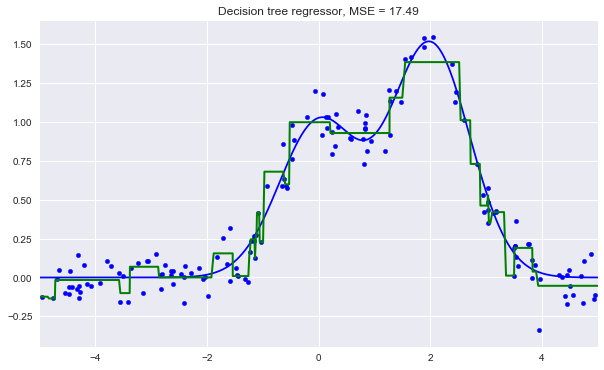
\includegraphics[width=\textwidth]{reg_tree}\caption{Решающее дерево в задаче регрессии}
		\end{figure}
	\subsection{Задача классификации}
		Обозначим за $p_{jk}$ долю объектов класса $c\in Y$ в многомерном прямоугольнике $R_j\in\mathbb R^p$ $$\widehat p_{jc}=\frac1{N_j}\sum\limits_{x_i\in R_j}\mathbbm{1}(y_i=c)$$.
		
		$\{R_j\}_{j=1}^J$~--- решение оптимизационной задачи $$\mathrm{ME}=1-\max_{j,c}\widehat p_{jc}\to\min\limits_{R_1,\ldots,R_J}.$$
		
		Однако $\mathrm{ME}$ не является дифференцируемой функцией(?вроде дифференцируемость и не нужна при построении), поэтому используются другие функции:
		\begin{itemize}
			\item Индекс Джини $G(j)=\sum\limits_{k=1}^K\widehat p_{jc}(1-\widehat p_{jc})$
			\item Кросс-энтропия $CI(j)=-\sum\limits_{k=1}^K\widehat p_{jc}\log\widehat p_{jc}$
		\end{itemize}
		
		\begin{figure}[h!]
		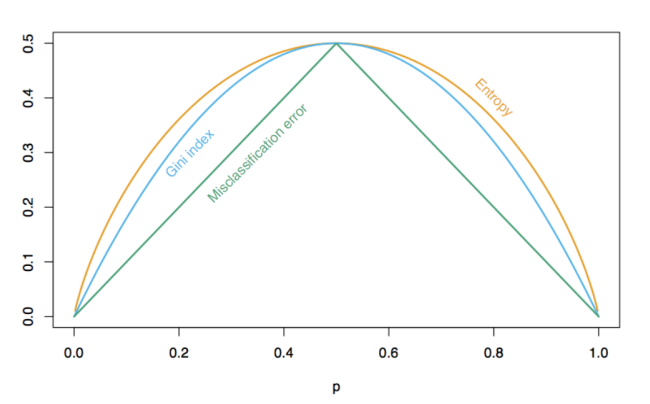
\includegraphics[width=\textwidth]{entr}\caption{Информационные индексы $ME$, $G$, $CI$ в случае двух классов}		
		\end{figure}
		
		Предсказание для объекта $x\in X$ равно $$f(x)=\argmax\limits_{c\in Y}\widehat{p}_{ck},$$ где $j$~--- индекс многомерного многоугольника, в который попадает $x$.
		
		\begin{figure}[h!]
		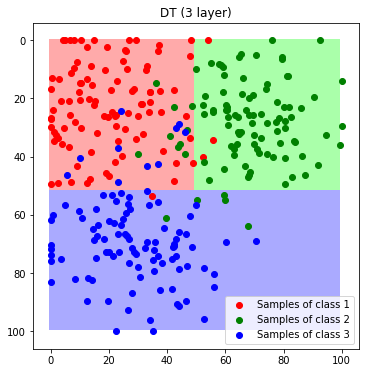
\includegraphics[width=\textwidth]{class_tree1}\caption{Решающее дерево в задаче классификации}		
		\end{figure}
	\subsection{Алгоритм построения дерева}
		\begin{enumerate}
			\item Выбираем признак $X_j$ и порог $s$ так, чтобы разбиение $X^n$ на\\$R_1(j,s) = \{x \in X^n | X_j <s\}$ и $R_2(j,s) = \{x \in X^n | X_j \ge s\}$ решало оптимизационную задачу, соответствующую задаче классификации или регрессии:
$$\sum\limits_{i: x_i \in R_1(j,s)}\mathrm{error}(y_i,\hat{y}_{R_1}) + \sum\limits_{i: x_i \in R_2(j,s)}\mathrm{error}(y_i,\hat{y}_{R_2}) \to \min\limits_{j,s},$$
где $\mathrm{error}$~--- функция потерь, в случае регрессии сумма остатков, в случае классификации индекс Джини или кросс-энтропия.
%\begin{equation*}
%\resizebox{.95\hsize}{!}{$\sum\limits_{i: x_i \in R_1(j,s)}\left(y_i - \frac{1}{|R_1|}\sum\limits_{l: x_l \in R_1(j,s)}y_l\right)^2 + \sum\limits_{i: x_i \in R_2(j,s)}\left(y_i - \frac{1}{|R_2|}\sum\limits_{l: x_l \in R_2(j,s)}y_l\right)^2$}
%\end{equation*}
\item Разбиваем выборку на области $R_1$ и $R_2$, образуя две дочерние вершины.
\item Повторяем процедуру в пределах каждой получаемой области, пока не выполнится критерий остановки.
\end{enumerate}

Очевидный критерий остановки~--- остановка в случае если все индивиды в листе принадлежат одному классу. Дополнительно можно задать следующие критерии остановки:
	\begin{itemize}
		\item Ограничение максимальной глубины дерева
		\item Ограничение минимального числа объектов в поддереве
		\item Информативность равна или меньше определенного значения
		\item Ограничение максимального числа индивидов в листе
	\end{itemize}
	
	\subsection{Обработка категориальных данных}
		Можно разбить вершину по категориям, однако такой подход может давать слишком глубокие деревья. Есть другой способ обработки категориальных значений, пусть категориальный признак имеет $M$ значений $\mathbb S=\{s_i\}_{i=1}^M$, будем рассматривать всевозможные разбиения $\mathbb S$ на 2 дизъюнктных подмножества $\mathbb S=V\cup W$, $V\cap W=\emptyset$. В таком случае предикат в вершине есть $\mathbbm{1}(x\in V)$. Проблема такого подхода заключается в том, что нужно перебрать $2^{M-1}-1$ разбиений, но есть алгоритм, позволяющий избавиться от перебора всех множеств и дающий результат, совпадающий с результатом полного перебора.
	
	\subsection{Обработка пропусков}
		Есть несколько способов обработки пропусков:
		\begin{itemize}
			\item Убрать индивидов с пропусками (pairwise). Однако после выкидывания всех пропусков, размер выборки может сильно уменьшиться.
			\item На стадии выбора разбиения пропуски не учитываются и значения с пропусками спускаются в одно поддерево
			\item Не учитывать на шаге поиска разбиения пропуски, но спустить индивидов в оба поддерева с весами
		\end{itemize}
	\newpage
	\subsection{ Преимущества и недостатки}
		\begin{figure}[h!]
			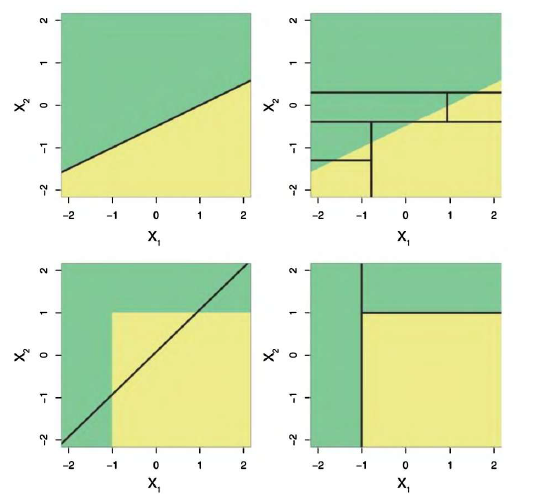
\includegraphics[width=\textwidth]{linreg_vs_tree}\caption{Примеры решений задач классификации с линейной (верхний ряд) и нелинейной (нижний ряд) зависимостью. В левой части решение с помощью линейной модели, в правой --- с помощью  решающего дерева.}
		\end{figure}
		Преимущества:
\begin{itemize}
\item  Простота интерпретации
\item  Пригодность и для задач регрессии, и для задач классификации
\item  Возможность работы с пропусками в данных
\end{itemize}
Недостатки:
\begin{itemize}
\item Основан на <<жадном>> алгоритме (решение является лишь локально оптимальным в каждом узле и может быть неоптимальным для всего дерева)
\item Метод явялется неустойчивым и склонным к переобучению
\end{itemize}
\newpage

\section{Вероятностная постановка}

\subsection{Генеральная постановка}

Предполагаем, что $\eta$ и $\bm{\xi}$ функционально зависимы:
\begin{equation}
	\eta = \varphi(\bm{\xi}) + \varepsilon,
\end{equation}
$\varphi$ --- неизвестная функция.\\
$\eta \in \mathbb{R}$ --- случайная величина, зависимая переменная.\\
$\bm{\xi} \in \mathbb{R}^p$ --- случайный вектор, признаки.\\
$\varepsilon \in \mathbb{R}$ --- случайная величина, ошибка.\\

\subsection{Выборочная постановка}

\begin{equation}
	y_i = \varphi(\textbf{x}_i) + \varepsilon_i,
\end{equation}
\noindent$\varphi$ --- неизвестная функция.\\
$y_i$ --- реализация случайной величины $\eta$, зависимая переменная.\\
$\textbf{x}_i$ --- реализация случайного вектора $\bm{\xi}$, признаки.\\
$\varepsilon_i \in \mathbb{R}$ --- реализация случайной величины $\varepsilon$, ошибка.\\

\newpage

\section{Алгоритмы}

\subsection{CART (использует Индекс Джини)}

\noindent Выбираем признак $X_j$ и порог $s$ так, чтобы разбиение $\textbf{X}$ на
$$R_1(j,s) = \{ \textbf{x}_i \in \textbf{X} | X_j < s \}$$
и
$$R_2(j,s) = \{ \textbf{x}_i \in \textbf{X} | X_j \geq s \}$$
решало задачу
\begin{equation}
	\sum\limits_{i:\textbf{x}_i \in R_1 (j,s)} (y_i - \hat{c}_1) + 	\sum\limits_{i:\textbf{x}_i \in R_2 (j,s)} (y_i - \hat{c}_2) \to \min_{j,s}
\end{equation}
где оценка коэффициента $\hat{c}_j = \dfrac{1}{|R_j|} \sum\limits_{\textbf{x}_i \in R_j(j,s)} y_i, \quad j = 1,2.$\\

\begin{enumerate}
	\item Перебираем все возможные $s_j$ и выбираем то значение, при котором Индекс Джини минимален.
	\item Разбиваем выборку на области $R_1$ и $R_2$, образуя две дочерние вершины $L_v$ и $R_v$.
	\item Повторяем процедуру, разбивая каждый из получившихся регионов, пока не будет достигнута максимальная глубина.
	\item Алгоритм CART --- жадный, он выбирает наилучшее расщепление на текущем уровне, что не обязательно приводит к наименьшей загрязненности на уровнях ниже. Алгоритм хорош, но не всегда оптимален.
\end{enumerate}

\subsection{ID3 (использует Кросс-энтропию)}

Идея алгоритма заключается в последовательном дроблении выборки на две части
до тех пор, пока в каждой части не окажутся объекты только одного класса. Нам необходимо выбирать такой предикат, чтобы ветвление дерева было максимально информативно

\begin{enumerate}
	\item $\textbf{X}$ --- обучающая выборка, $\textbf{y} \in \{1, \cdots, k\}$.
	\item Если все $\textbf{x}_i$ имеют класс $k$, ставим метку 1 в корень и выходим из цикла.
	\item Если ни один $\textbf{x}_i$ не имеет класс $k$, ставим метку 0 в корень и выходим из цикла.
	\item Предикат $R(\textbf{x}_i):=\{ \textbf{x}_i | X_j \lessgtr s_j \}$ для которого информационная выгода наибольшая.
	\item Разбиваем $\textbf{X}$ на $\textbf{X}_0$ и $\textbf{X}_1$ по предикату $R$
	$$\textbf{X}_0:=\{ \textbf{x}_i \in \textbf{X}:R(\textbf{x}_i) = 0 \},$$
	$$\textbf{X}_1:=\{ \textbf{x}_i \in \textbf{X}:R(\textbf{x}_i) = 1 \}.$$
	\item Если $\textbf{X}_0 = \varnothing$ или $\textbf{X}_1 = \varnothing$, создаем новый лист $v$, $k_v$ --- класс, в котором находится большинство элементов $\textbf{x}_i.$
	\item Иначе создаем внутреннюю вершину $v$:
	\begin{enumerate}
		\item $R_v = R$;
		\item $L_v$;
		\item $R_v$.
	\end{enumerate}
\end{enumerate}

\subsection{Стрижка деревьев}

Описанный выше процесс может дать хорошие прогнозы на обучающем наборе, но, вероятно, \textit{переобучится}, что приведет к плохим результатам на тестовых наборах. Почему?

Меньшее дерево с меньшим количеством разбиений (то есть с меньшим количеством областей $R_1, \cdots, R_J$) может привести к меньшей дисперсии и лучшей интерпретации за счет небольшого смещения. Мы можем пожертвовать смещением, но получить меньшую дисперсию.

Одна из возможных альтернатив описанному выше процессу --- выращивать дерево только до тех пор, пока уменьшение RSS из-за каждого разбиения превышает некоторый (высокий) порог.

Эта стратегия приведет к уменьшению размеров деревьев, но она слишком недальновидна: за кажущимся бесполезным разбиением в начале дерева может последовать очень хорошее разбиение --- то есть разделение, которое в дальнейшем приводит к значительному сокращению RSS.

Лучшая стратегия --- вырастить очень большое дерево $T_0$, а затем обрезать его, чтобы получить поддерево.

\textit{Cost complexity prunning} --- также называется сокращением наиболее слабых звеньев --- используется для этого.

Мы рассматриваем последовательность деревьев, с настраиваемыми параметрами $\alpha$. Каждому значению $\alpha$ соответствует поддерево $T \subset T_0$ (является подмножеством) такое, что
\begin{equation}
	\sum\limits_{j=1}^{|T|} \sum\limits_{\textbf{x}_i \in R_j}^{} (y_i - \hat{y}_{R_j})^2 + \alpha |T|.
\end{equation}
настолько мало насколько это возможно. Здесь $|T|$ указывает количество конечных узлов дерева $T$, $R_j$ --- это прямоугольник (\textbf{то есть подмножество пространства предикторов}), соответствующий $j$-му конечному узлу, а $\hat{y}_{R_j}$ --- это среднее значение обучающих наблюдений в $R_j$.

\textbf{Критерий остановки}:\\
1. Ограничение макс. глубины дерева;\\
2. Ограничение мин. числа объектов в листе $n_{min}$;\\
3. Ограничение макс. количества листьев в дереве;\\
4. Остановка в случае, если все объекты в листе относятся к одному классу.

\newpage

\section{Бутстрап}

Пусть дана конечная выборка $X = (x_i,y_i)$ с вещевственными ответами. Сгенерируем подвыборку с помощью бутстрапа. Равномерно возьмем из выборки $l$ объектов с возвращением. Отметим, что из-за возвращения среди них окажутся повторы. Обозначим новую выборку через $X_1$. Повторим процедуру $N$ раз и получим подвыборки $X_1,\ldots,X_N$. Обучим по каждой выборке модель линейной регрессии и получим базовые алгоритмы $b_1(x),\ldots,b_N(x)$.

Предположим, что существует истинная функция ответов для всех объектов $y(x)$ и задано распределение на объектах $p(x)$. Тогда мы можем записать ошибку каждой функции регрессии, как 

\begin{equation}
	\epsilon_j(x)=b_j(x)-y(x),\space j = 1,...,N,
\end{equation}

и записать матожидание среднеквадратичной ошибки:

\begin{equation}
	\mathbb{E}_x\left(b_j(x) - y(x)\right)^2 = \mathbb{E}_x\epsilon^2_j(x)
\end{equation}

Средняя ошибка построенных функций регрессии имеет вид

$E_1= \dfrac{1}{N}\sum_{j=1}^{N}\mathbb{E}_x\epsilon^2_j(x)$

Предположим, что ошибки несмещены и некоррелированы:

$\mathbb{E}_x\epsilon_j(x) = 0$

$ \mathbb{E}_x\epsilon_i(x)\epsilon_j(x) = 0$,  $i\neq j$

Построим  новую функцию регрессии, которая будет усреднять ответы построенных нами функций:

$a(x) = \frac{1}{N}\sum_{j=1}^{N}b_j(x)$

Ее среднеквадратичная ошибка:

$E_N = \mathbb{E}_x\left(\frac{1}{N}\sum_{j=1}^{N}b_j(x)-y(x)\right)^2 = \mathbb{E}_x\left(\frac{1}{N}\sum_{j=1}^{N}\epsilon_j(x)\right)^2 = $

$=\frac{1}{N^2}\mathbb{E}_x\left(\sum_{j=1}^{N}\epsilon^2_j(x) + \sum_{i\neq j}^{}\epsilon_i(x)\epsilon_j(x)\right)=\frac{1}{N}E_1$

Усреднение ответов позволило уменьшит средний квадрат ошибки в $N$ раз.

Это является идеальным случаем, так как на практике некоррелируемость ошибок редко случается.

\section{Bias-Variance decomposition}

Ошибка любой модели складывается из трех факторов: сложности самой выборки, сходства модели с истинной зависимостью ответов от объектов в выборке, и богатства семейства, из которого выбирается конкретная модель. Между этими факторами существует некоторый баланс, и уменьшение одного из них приводит к увеличению другого. Такое разложение ошибки носит название разложения на смещение и разброс.

Пусть задана выборка $X = (x_i,y_i)^l_{i=1}$ с вещественными ответами $y_i \in \mathbb{R}$. Будем считать что на пространстве $\mathbb{X} \times \mathbb{Y}$ существует распределение $p(x,y)$, из которого сгенерирована выборка $X$ и все ответы на ней.

Рассмотрим квадратичную функцию потерь $L(y,a) = (y-a(x))^2$ и ее среднеквадратичный риск

$R(a) = \mathbb{E}_{x,y}\left[(y-a(x))^2\right] \int_{\mathbb{X}}\int_{\mathbb{Y}} p(x,y)(y-a(x))^2dxdy$

Такой функционал усредняет ошибку модели в каждой точке пространства $x$ и для каждого возможного ответа $y$, причём вклад пары $(x, y)$, по сути, пропорционален вероятности получить её в выборке $p(x, y)$. Разумеется, на практике мы не можем вычислить данный функционал, поскольку распределение $p(x, y)$ неизвестно. Тем не менее, в теории он позволяет измерить качество модели на всех возможных объектах, а не только на обучающей выборке.

\subsection{Минимум среднеквадратичного риска}

???

\subsection{Ошибка метода обучения}

Для того, чтобы построить идеальную функцию регрессии, необходимо знать распределение на объектах и ответах $p(x, y)$, что, как правило, невозможно. На практике вместо этого выбирается некоторый метод обучения $\mu : (\mathbb{X}\times\mathbb{Y})^l \rightarrow \mathbf{A}$, который произвольной обучающей выборке ставит в соответствие некоторый алгоритм из семейства $\mathbf{A}$. В качестве меры качества метода обучения можно взять усредненный
по всем выборкам среднеквадратичный риск алгоритма, выбранного методом $\mu$ по ввыборке:

\begin{multline}
	L(\mu) = \mathbb{E}_X\left[\mathbb{E}_{x,y}\left[ \left(y-\mu(X)(x))\right)^2\right]\right] =  \\ =\int_{(\mathbb{X}\times\mathbb{Y})^l}\int_{\mathbb{X}\times\mathbb{Y}} \left(y-\mu(X)(x)\right)^2 p(x,y)\prod^l_{i=1}p(x_i,y_i)dxdydx_1dy_1,\ldots dx_ldy_l
	\label{risk}
\end{multline}

Здесь матожидание $\mathbb{E}_X[\cdot]$ берется по всем возможным выборкам ${(x_1, y_1), . . . ,(x_l, y_l)}$
из распределения $\prod_{i=1}^{l}p(x_i,y_i)$.

Среднеквадратичный риск на фиксированной выборке X можно расисать как

$\mathbb{E}_{x,y} = \left[(y-\mu(X))^2\right] = \mathbb{E}_{x,y}\left[(y-\mathbb{E}[y|x])^2\right] + \mathbb{E}_{x,y}\left[(\mathbb{E}[y|x] - \mu(X))^2\right]$

Подставим эту формулу в (\ref{risk}).

\begin{equation}
	\begin{split}
	L(\mu) = \mathbb{E}_X\left[\underbrace{\mathbb{E}_{x,y}\left[(y-\mathbb{E}[y|x])^2\right]}_{\text{не завсисит от X}} + \mathbb{E}_{x,y}\left[(\mathbb{E}[y|x] - \mu(X))^2\right]\right] = \\
	= \mathbb{E}_{x,y}\left[(y-\mathbb{E}[y|x])^2\right] + \mathbb{E}_{x,y}\left[\mathbb{E}_X \left[(\mathbb{E}[y|x]- \mu(X))^2\right]\right]
\end{split}
\label{2.2}
\end{equation}
Преобразовываем второе слагаемое:


\begin{multline}
	\mathbb{E}_{x,y}\left[\mathbb{E}_X \left[(\mathbb{E}[y|x] - \mu(X))^2\right]\right] = \\ = \mathbb{E}_{x,y}\left[\mathbb{E}_X \left[(\mathbb{E}[y|x] - \mathbb{E}_X[\mu(X)] + \mathbb{E}_X[\mu(X)] -\mu(X))^2\right]\right] = \\ =
	\mathbb{E}_{x,y}\left[\mathbb{E}_X \left[\underbrace{(\mathbb{E}[y|x] - \mathbb{E}_X \mu(X))^2}_{\text{не завсисит от X}}\right]\right] + \mathbb{E}_{x,y}\left[\mathbb{E}_X \left[(\mathbb{E}_X \mu(X) - \mu(X))^2\right]\right] + \\ + 
	2\mathbb{E}_{x,y} \left[\mathbb{E}_X\left[(\mathbb{E}[y|x] - \mathbb{E}[\mu(X)])(\mathbb{E}_X[\mu(X)]-\mu(X))\right]\right]
	\label{2.3}
\end{multline}

Последнее слагаемое обращается в ноль.

Подставим (\ref{2.3}) в \ref{2.2}.

\begin{multline}
	L(\mu) = \underbrace{\mathbb{E}_{x,y}\left[(y-\mathbb{E}[y|x])^2\right]}_{\text{шум}} + \\ +
	\underbrace{\mathbb{E}_x\left[\left(\mathbb{E}_X[\mu(X)] - \mathbb{E}[y|x]\right)^2\right]}_{\text{смещение}} + \underbrace{\mathbb{E}_x\left[\mathbb{E}_X\left[(\mu(X) - \mathbb{E}_X[\mu(X)])^2\right]\right]}_{\text{разброс}}
	\label{2.4}
\end{multline}

Первая компонента характеризует шум в данных и равна ошибке идеального алгоритма. Невозможно построить алгоритм, имеющий меньшую среднеквадратичную ошибку. Вторая компонента характеризует смещение (bias) метода обучения, то есть отклонение среднего ответа обученного алгоритма от ответа идеального алгоритма. Третья компонента характеризует дисперсию (variance), то есть разброс ответов обученных алгоритмов относительно среднего ответа. 

Смещение показывает, насколько хорошо с помощью данных метода обучения и семейства алгоритмов можно приблизить оптимальный алгоритм. Как правило, смещение маленькое у сложных семейств (например, у деревьев) и большое у простых семейств (например, линейных классификаторов). Дисперсия показывает, насколько сильно может изменяться ответ обученного алгоритма в зависимости от выборки --- иными словами, она характеризует чувствительность метода обучения к изменениям в выборке. Как правило, простые семейства имеют маленькую дисперсию, а сложные семейства --- большую дисперсию.


\begin{figure}[!ht]
	\centering
	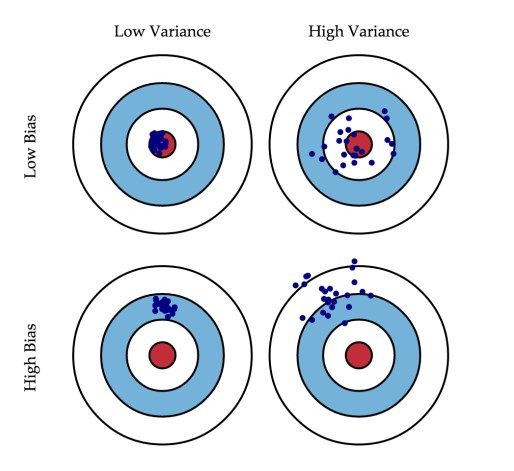
\includegraphics[width=1\textwidth]{bias_var.jpg}
	\caption{Сдвиг и разброс разных моделей}
	\label{fig:bias_var}
\end{figure}


На рис. \ref{fig:bias_var} изображены модели с различными сдвигом и разбросом. Модели изображены синими точками, одна точка соответствует модели, обученной по одной из возможных обучающих выборок. Каждый круг характеризует качество модели --- чем ближе точка к центру, тем меньше ошибок на контрольной выборке достигает данный алгоритм. Видно, что большой сдвиг соответствует тому, что в среднем точки не попадают в центр, то есть в среднем они не соответствуют лучшей модели.

Большой разброс означает, что модель может попасть по качеству куда угодно --- как в центр, так и в область с большой ошибкой.

\section{Bagging}

Деревья решений, страдают от высокой дисперсии. Это означает, что если разделить обучающие данные на две части случайным образом и применить дерево решений к обеим половинам, результаты, которые мы получим, могут быть совершенно разными. Напротив, процедура с низкой дисперсией даст схожие результаты при многократном применении к разным наборам данных; линейная регрессия имеет тенденцию к низкой дисперсии, если отношение $n$ к $p$ умеренно велико. Бэггинг, --- это процедура для уменьшения дисперсии статистического метода обучения; она особенно полезна и часто используется в контексте деревьев решений.

Пусть у нас имеется набор из $n$ независивых наблюдений $X_1,\ldots X_n$, каждый из которых имеет дисперсию $\sigma^2$, дисперсия $\bar{X}$ будет равна $\sigma^2/n$. Другими словами, усреднение набора наблюдений снижает дисперсию.

Следовательно, естественный способ уменьшить дисперсию и, следовательно, увеличить точность предсказания статистического метода обучения заключается в том, чтобы взять множество обучающих наборов из выборки, построить отдельную модель предсказания, используя каждый набор обучения и усреднить полученные прогнозы. 

\begin{equation}
	{a}_{N}(x) = \dfrac{1}{N}\sum_{n=1}^{N}\hat{\mu}(x)
\end{equation}

Однако на практике это не реализовать, потому что у нас нет нескольких сетов обучающих данных. Вместо этого, мы можем примеить бутстрап беря несколько сэмплов из обучающего набора данных. При таком подходе, мы генерируем $B$ разных подвыборок с помощью бутсрапа. Затем мы обучаем модель на $b$-ом сете обучающих данных и усредняем прогнозы.

Это называется бэггингом.

Заметим, что в методе обучения для бэггинга появляется ещё один источник случайности — взятие подвыборки. Чтобы функционал качества $L(\mu)$ был детерминированным, мы будем далее считать, что матожидание$ \mathbb{E}_X [\cdot]$ берётся не только по всем обучающим выборкам $ X$, но ещё и по всем возможным подвыборкам $\hat{X}$, получаемым с помощью бутстрапа. Это вполне логичное обобщение, поскольку данное матожидание вводится в функционал именно для учёта случайностей, связанных с процедурой обучения модели.

Найдём смещение из разложения (\ref{2.4}) для бэггинга:

\begin{multline}
	\mathbb{E}_{x,y}\left[\left(\mathbb{E}_X\left[\frac{1}{N}\sum_{b=1}^{N}\hat{\mu}(X)(x)\right]-\mathbb{E}[y|x]\right)^2\right] = \mathbb{E}_{x,y}\left[\left(\frac{1}{N}\sum_{b=1}^{N}\mathbb{E}_X[\hat{\mu}(X)(x)] - \mathbb{E}[y|x]\right)^2\right] = \\ =\mathbb{E}_{x,y}\left[(\mathbb{E}_X\left[\hat{\mu}(X)(x)\right]-\mathbb{E}[y|x])^2\right]
\end{multline}


Мы получили, что смещение композиции, полученной с помощью бэггинга, совпадает со смещением одного базового алгоритма. Таким образом, бэггинг не ухудшает смещенность модели.

Теперь рассмотрим разброс. Из (\ref{2.4}) он равен:

\begin{multline}
	\frac{1}{N}\mathbb{E}_{x,y}\left[\mathbb{E}_X\left[\left(\hat{\mu}(X)(x)-\mathbb{E}_X[\hat{\mu}(X)(x)]\right)^2\right]\right] + \\ + 
	\frac{N(N-1)}{N^2}\mathbb{E}_{x,y}\left[\mathbb{E}_X\left[\left(\hat{\mu}(X)(x)-\mathbb{E}_X[\hat{\mu}(X)(x)]\right)\times \left(\hat{\mu}(X)(x)-\mathbb{E}_X[\hat{\mu}(X)(x)]\right)\right]\right]
\end{multline}

Первое слагаемое — это дисперсия одного базового алгоритма, деленная на длину композиции $N.$ Второе --- ковариация между двумя базовыми алгоритмами. Мы видим, что если базовые алгоритмы некоррелированы, то дисперсия композиции в $N$ раз меньше дисперсии отдельных алгоритмов. Если же корреляция имеет место, то уменьшение дисперсии может быть гораздо менее существенным.

До сих пор мы описывали бэггинг в контексте регрессии, для предсказания количественного результата $y$. Как можно распространить бэггинг на задачу классификации, где $Y$ является качественным? В этой ситуации существует существует несколько возможных подходов, но самый простой заключается в следующем. Для тестового сета, мы можем записать класс, предсказанный каждым из $N$ деревьев, и сделать "\textit{majority vote}" --- это наиболее часто встречающийся класс среди $N$ предсказаний.

\subsection{Out-of-Bag Error Estimation}

Ключевой момент bagging модели заключается в том, что деревья многократно подгоняются к бутстреп-подмножествам наблюдений. В среднем каждое дерево сетки использует около двух третей наблюдений. Оставшаяся треть наблюдений, не использованная для подгонки данного дерева сетки, называется \textit{out-of-bag} наблюдениями (OOB).

Мы можем предсказать ответ для i-го наблюдения, используя каждое из деревьев, в которых это наблюдение было OOB. Это даст около N/3 предсказаний для i-го наблюдения. Для того чтобы получить единое предсказание для i-го  наблюдения, мы можем усреднить эти предсказанные ответы (при регрессионной модели) или взять majority vote (при классификации). Это приводит к единственному OOB-предсказанию для каждого наблюдения. Предсказание OOB может быть получено таким образом для каждого из $n$ наблюдений, из чего следует, что общий MSE OOB (для задачи регрессии) или ошибка классификации (для задачи классификации) может быть вычислена. Полученная ошибка OOB является достоверной оценкой тестовой ошибки для bagging модели, поскольку прогноз для каждого наблюдения предсказывается с использованием только тех деревьев, которые не подошли для данного наблюдения. 

$OOB = \sum_{i=1}^{l}L\left(y_i,\frac{1}{\sum_{n=1}^{N}\left[x_i \notin X_n\right]}\sum_{n=1}^{N}[x_i\notin X_n]b_n(x_i)\right)$


\end{document}